\chapter{Literature Review}
\label{ch:lit}

Although soundscape studies have seen increased attention over the last decade \citep{Kang2016Ten}, engineering practice is still dominated by a noise control approach. For this reason, this review of the literature will begin with some examples of how urban sound is assessed by standard noise control methods before moving on to discuss how the soundscape approach represents an improvement over these methods. From here, I will present the conceptual framework for predictive soundscape models \citep{Aletta2016Soundscape} from which the work in this thesis began and discuss why predictive models are necessary to enable an engineering approach to soundscape design. Finally, some tools and previous predictive models are reviewed.

\section{The importance of perception and experience}
Despite being the dominant focus of urban noise mitigation, the reduction of sound levels has been proven to not necessarily correlate with perception or lead to improved health outcomes \citep{Kang2006Urban,Andringa2013Positioning,Kempen2014Characterizing,Asdrubali2014New,Kang2016Ten}. Research from the early 2000s demonstrated that reducing the sound level does not necessarily lead to better acoustic comfort in urban areas \citep{DeRuiter2000Noise,SchulteFortkamp2001Quality}. \citet{Yang2005Acoustic} assessed the acoustic comfort of people in 14 urban spaces in five European countries (Greece, Italy, UK, Germany, and Switzerland). For this study, users of the space were randomly selected in the spaces and asked to evaluate the subjective sound level on a scale from 1 (very quiet) to 5 (very noisy), while an additional measure of acoustic comfort was assessed (from 1 [very comfortable] to 5 [very uncomfortable]) in the 2 case study sites in Sheffield, UK. While each participant was interviewed, the researchers measured the 1-minute \gls{laeq} as well as additional microclimate indices. 

By examining the relationship between the subjective sound level and the measured sound level within each site separately, their results indicated an inconsistent relationship across sites, with correlation values ranging from $R=0.373$ for Sesto San Giovanni, Italy to $R=0.941$ for Karaisakaki square, Greece. This indicates that although \gls{laeq} can be a good indicator for the subjective sound level, the strength of this relationship and in particular the slope of the relationship depends on other factors not captured by the decibel. This is further reinforced by the acoustic comfort results. \cref{fig:yang2005acousticComfort} shows the acoustic comfort and subjective sound level ratings for the two Sheffield case study sites reported in \citet{Yang2005Acoustic}. Although in these sites there is a strong correlation between the \gls{laeq} and the subjective sound level, the correlation with acoustic comfort is much weaker. In addition, \cref{fig:yang2005acousticComfort}(a) in particular shows a nonlinear relationship between dB(A) and acoustic comfort. It can be seen that above $\sim$70 dB(A) the acoustic comfort decreases as the sound level increases, however below 70 dB(A) there is no significant change in acoustic comfort. 

\begin{figure}
  \centering
  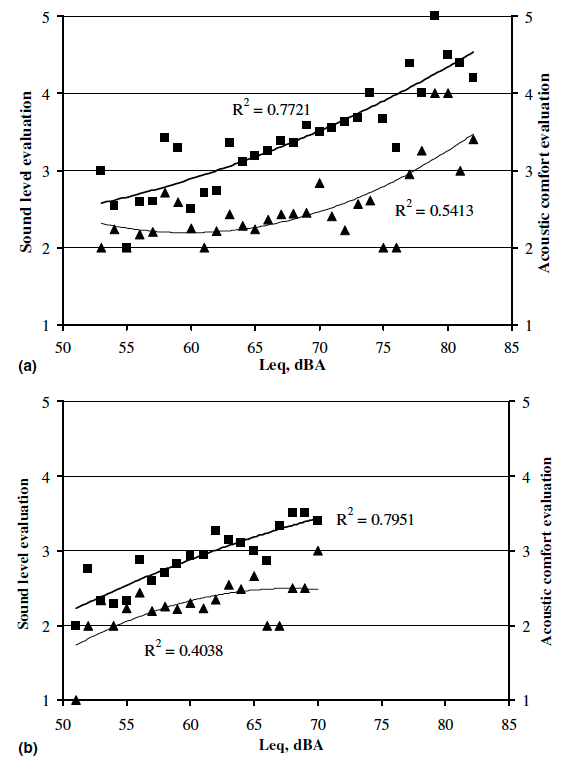
\includegraphics[width=.65\textwidth]{Figures/YangKang2005 Acoustic Comfort dB.png}
  \caption[Subjective responses and measured sound levels in urban spaces in Sheffield, UK.]{Reproduced with permission from \citep[Fig. 2]{Yang2005Acoustic} showing subjective responses and measured sound levels in urban spaces in Sheffield, UK. Relationships between the measured sound level, the mean subjective evaluation of the sound level and the mean acoustic comfort evaluation, with binomial regressions and correlation coefficients squared $R^2$. (a) The Peace Gardens. (b) The Barkers Pool. $\blacksquare$ -- subjective evaluation of sound level (1 [very quiet]; 2 [quiet]; 3 [neither quiet nor noisy]; 4 [noisy]; 5 [very noisy]). $\blacktriangle$ -- acoustic comfort evaluation (1 [very comfortable]; 2 [comfortable]; 3 [neither comfortable nor uncomfortable]; 4 [uncomfortable]; 5 [very uncomfortable]). \label{fig:yang2005acousticComfort} }
\end{figure}

\vspace{4mm}
\noindent\fbox{
    \parbox{\textwidth}{
      \vspace{-.25cm}
    \paragraph{Parallels in visual perception of green space}
    Similar results showing the disconnect between commonly used metrics of the physical environment and the environment's impact on the users have also been demonstrated by studies looking at visual perception. \citet{Kruize2019Exploring} demonstrated that the experience and use of natural urban spaces were strongly related to health outcomes associated with those spaces, while strictly physical characteristics of the space were not. 
    Their study made use of a cross-sectional design to investigate the relationships between several factors related to the experience of natural outdoor environments and key health outcome indicators. The outcome indicators investigated included physical activity, social contact, and mental health. As input indicators, they considered a set of GIS-derived quantitative indicators (i.e. \gls{ndvi}) \citep{Smith2017Characterisation} and a selection of metrics describing the use and experience of the space, derived from surveys of the study participants. These survey-derived experience metrics included \emph{perceived greenness}, \emph{satisfaction with the natural environment}, and \emph{importance of the natural environment}. Through multilevel regression analyses, the authors found that, in general, \gls{ndvi} was not statistically significantly related to increased physical activity or improved mental health, while perceived greenness, satisfaction with the space, and importance of the space were. A one point increase in perceived greenness (ranging from 0-12) was associated with an additional 10 min of physical activity per week and an increased mental well-being score (MHI-5) of 0.331 (range 8-100). 

    What is particularly interesting in these results is the difference in the findings between the objective measure of greenness and the perceived greenness. A study which used only the GIS-derived metric would have concluded that there was no relationship between greenness and the outcome factors. By including a perceptual attribute, \citet{Kruize2019Exploring} were able to demonstrate its importance. This suggests that what really matters to people's use of and the health and well-being impacts of these spaces is \emph{how they are perceived} more so than just what the physical characteristics. 
    }
}


\paragraph*{}Across both the visual and the auditory domain, research has suggested that a disconnect exists between the physical metrics used to describe urban environments and how they are perceived. In addition, this disconnect can be extended further into how these environments influence the health and well-being of their users. To gain a better understanding of these spaces and their impacts on people who work and live in cities, we must create assessment methods and metrics which go beyond merely characterising the physical environment and instead translate through the users' perception. In order to make the case for why a new approach to perception-focussed assessment and design is necessary, we must first understand how the existing assessment methods have attempted to consider perception.


\section{Attempts to reconcile dB-focussed noise control with human perception}
In this section, I will begin with a brief discussion of the noise approach to annoyance and review some examples of noise assessment and mitigation methods and how they have attempted to reconcile the noted disconnect between the dB and the sound perception. This will provide the existing context for how traditional noise control approaches are targeted. 

\subsection{Assessing noise} In the UK, \citet{BS41422019} is the current reference document for assessing and addressing noise impacts in outdoor environments. In particular, BS 4142 is intended to assess the impact of a specific noise source when introduced to a given background level. BS 4142 makes use of a `rating level' based on a comparison between the sound which is being assessed and the background sound which would exist without it. Within the standard, a series of noise metrics are defined \citep[Sec. 3]{BS41422019}:

\begin{itemize}
  \item \textbf{ambient sound level, $L_a = L_{Aeq,T}$} - equivalent continuous A-weighted sound pressure level of the totally encompassing sound in a given situation at a given time, usually from many sources near and far, at the assessment location over a given time interval, \emph{T}.
  \item \textbf{background sound level, $L_{A90,T}$} - A-weighted sound pressure level that is exceeded by the residual sound at the assessment location for 90\% of a given time interval, \emph{T}, measured using time weighting, \emph{F}, and quoted to the nearest whole number of decibels.
  \item \textbf{equivalent continuous A-weighted sound pressure level, $L_{Aeq,T}$} - value of the A-weighted sound pressure level in decibels of continuous steady sound that, within a specificed time interval, $T = t_2 - t_1$, has the same mean-squared sound pressure as a sound that varies with time, and is given by the following equation:
  \begin{equation}
    L_{Aeq,T} = 10 lg_{10} \left[\frac{1}{T} \int^{t_2}_{t_1} \frac{p_A(t)^2}{p_0^2}dt \right]
  \end{equation}
    where: \\
      \space $p_0$ is the reference sound pressure (20 $\mu Pa$); and\\
      \space $p_a{t}$ is the instantaneous A-weighted sound pressure (Pa) at time \emph{t}
  \item \textbf{residual sound level, $L_r=L_{Aeq,T}$} - equivalent continuous A-weighted sound pressure level of the residual sound\footnote{Ambient sound remaining at the assessment location when the specific sound source is suppressed to such a degree that it does not contribute to the ambient sound.} at the assessment location over a given time interval, \emph{T}.
  \item \textbf{specific sound level, $L_s=L_{Aeq,Tr}$} - equivalent continuous A-weighted sound pressure level produced by the specific sound source at the assessment location over a given reference time interval, $T_R$.
\end{itemize}

In each of these metrics, the primary sonic feature which is assessed is the sound level, with some consideration for frequency content by using A-weighting. The standard then sets out the procedure to be used to measure the existing background sound level, measure or estimate the level of the specific sound, and calculate the margin between the specific sound and the background sound level. Throughout this process, BS 4142 notes `certain acoustic features can increase the significance of impact over that expected from a basic comparison between the specific sound level and the background sound level.' To address this, it introduces certain methods to add a character correction to the specific sound level, resulting in the rating level:

\begin{itemize}
  \item \textbf{rating level, $L_{Ar,Tr}$} - specified sound level plus any adjustment for the characteristic features of the sound
\end{itemize}

The sonic characteristics included for these rating level adjustments are tonality, impulsivity, intermittency, and `other sound characteristics' (described as `otherwise readily distinctive against the residual acoustic environment'). As an example of how these adjustments are applied, I will quote the guidance to adjust for tonality:
%\citep[pg. 13]{BS41422019}:

\begin{quote}
  \textbf{Tonality} \\
  For sound ranging from not tonal to prominently tonal the Joint Nordic Method \citep{ISO1996Part1} gives a correction of between 0 dB and + 6 dB for tonality. Subjectively, this can be converted to a penalty of 2 dB for a tone which is just perceptible at the noise receptor, 4 dB where it is clearly perceptible, and 6 dB where it is highly perceptible.
      \begin{flushright}
    \citet[pg. 13]{BS41422019}
  \end{flushright}
\end{quote}

The goal of these rating level adjustments is to incorporate aspects of the specific perception of sound, which may make a sound more disturbing, more noticeable, or generally more impactful than the dBA value alone would suggest. This is an important part of rating the impact of these sounds and necessary to achieve the goals of the standard. However, by implementing this as adjustments in terms of dB, it still centres the sound level in the assessment and enables only a one-dimensional approach to assessing impact. 

While BS 4142 is targeted towards assessing the impact of a specific sound, and primarily in an industrial and commercial context, \citet{ISO1996Part1} is more general, including provisions for assessing `community noise'. In the Introduction to the standard, several acknowledgements are raised about the importance of human perception, but the primary focus on the sound level is confirmed:

\begin{quote}
  To be of practical use, any method of description, measurement, and assessment of environmental noise is intended to be related in some way to what is known about human response to noise. [\ldots] The methods and procedures described in this part of ISO 1996 are intended to applicable to noise from various sources, individually or in combination, which contribute to the total exposure at a site. At the stage of technology at the time of publication of this part of ISO 1996, the evaluation of long-term noise annoyance seems to be best met by adopting the adjusted A-weighted equivalent continuous sound pressure level, which is termed a ``rating level''. 
        \begin{flushright}
    \citet{ISO1996Part1}
  \end{flushright}
\end{quote}

Despite the nods toward a perception-focussed approach, ISO 1996 re-emphasises the focus on sound pressure level when it comes to discussing community noise annoyance:

\begin{quote}
  If the sound has special characteristics, then the rating equivalent continuous sound pressure level shall be the primary measure used to describe the sound. [\dots] research has shown that different transportation sounds or industrial sounds evoke different community annoyance responses for the same A-weighted equivalent continuous sound pressure level.
        \begin{flushright}
    \citet[Sec. 6.1]{ISO1996Part1}
  \end{flushright}
\end{quote}

What this review of some of the relevant standards and guidance demonstrates is that the decibel (specifically the equivalent continuous sound pressure level) is the dominant rating metric for all types of environmental noise and that, despite attempts to incorporate adjustments for `special' characteristics of the sound, the only sonic characteristic really being considered is the sound level. In addition, what my review of this guidance reveals is that the rating level adjustments are impractical to apply to complex sound environments for general evaluation. \citet[Eq. 4]{ISO1996Part1} provides a formula for calculating the rating level of combined sources:

\begin{equation}
L_{Req,T} = 10lg \left(\frac{1}{T} \sum_n \sum_j T_{nj} * 10^{0,1L_{Reqj,Tnj}}  \right) dB
\label{eqn:iso1996Rating}
\end{equation}
where

$$
T = \sum_n T_{nj}
$$

for each source \emph{j}.

However, ISO 1996 notes that `As a practical matter, [\cref{eqn:iso1996Rating}] is typically evaluated one source at a time.' This makes it clearly impractical as a method for assessing a general sound environment, with multiple competing sound sources, or for automated monitoring. In this way, these standards preclude the possibility of making use of the rating level to provide a more nuanced view of a sound environment which accounts for the sonic characteristics. 

\subsection{Community noise annoyance}
There is an existing methodology to address community noise annoyance, which began to develop in the 1940s following an increase in community complaints, primarily in response to aircraft noise \citep{Kryter1994}\footnotemark{}. From this, definitions of noise annoyance and single-number assessment indices were developed which focussed on the aircraft and transport noise impacts on residential areas. \citet{ISO15666} defines annoyance (specifically `noise-induced annoyance') as `one person's individual reaction to noise.` This is assessed through socio-acoustic surveys using questions with either verbal or numerical rating scales. In contrast to many studies from the soundscape literature, the noise annoyance scales in \citet{ISO15666} refer to long time scales (`Thinking about the last (12 months or so) \ldots') whereas soundscape studies have tended to focus on shorter and more immediate time scales \citep{Yang2013Psychoacoustical,Rychtarikova2013Soundscape}. This is perhaps due to the more complex nature of the perception under investigation in soundscape. 

\citet{ISO15666} then extends to \emph{community noise annoyance}, defined as `the prevalence rate of this individual reaction in a community as measured by the responses to questions specified in Clause 4 and expressed in appropriate statistical terms.' This approach to community noise inherently recognises that 1) noise annoyance is an individual response which will vary among people and 2) the most appropriate way to discuss this impact on a broader scale is to describe the aggregate response statistically (e.g. 80\% prevalence of `highly annoyed' individuals).

A commonly used metric in noise annoyance studies in this context is the \gls{ldn}, which is the average of the sum of the A-weighted sound energy over 24 hours, with a penalty of 10 dB added for the hours from 10:00 pm to 7:00 am, on an annualised basis \citep[pg. 571]{Kryter1994}:

\begin{dmath}
  L_{dn} = 10 log((1/54,000 (10^{L_{A}1s,7am..L_A1s,10pm/10})\\ + (10(1/32,400 (10^{L_A1s,10pm..L_A1s,7am/10}))
\end{dmath}


In the contexts for which it was developed, \gls{ldn} provides a good correlation with `the cumulative percentage of people' being moderately, very, or highly annoyed for specific sources of noise, such as aircraft noise (0.89, 0.89, and 0.87, respectively) \citep{Kryter1994}. A predictive trend curve can be derived from this:

\begin{equation}
\% \text{Highly annoyed} = 110.091 + (-5.023 \times L_{dn}) = (0.058 \times L_{dn}^2)
\end{equation}

However, as noted, this is employed for assessing the annualised annoyance from a particularly noted source averaged over 24 hours in a residential setting. The residential setting is particularly noted in the inclusion of the 10 dB penalty during night-time hours, to consider sleep disturbance impacts. The long time-scales and the and lack of consideration of either more complex sonic characteristics or the potential positive impacts of sounds make these methods unsuitable for assessing the soundscape of public spaces. However, noise annoyance methodology does provide a valuable advantage for our purposes when compared to the environmental noise assessment methods reviewed earlier:

\begin{quote}
  The procedures for estimating subjective annoyance and complaints about environmental noise are intended for the assessment of the reactions of large groups or neighborhoods of people, and not specific individuals within a group.
  \begin{flushright}
    \citet[pg. 571]{Kryter1994}
  \end{flushright}
\end{quote}

This concept will be further explored and addressed in \cref{ch:ProbabilisticPOC}.

\footnotetext{\citet{Kryter1994} opts not to refer to annoyance when referring to a single sound, in order to `avoid some of the ambiguity possible with the word \emph{annoyance}'. Instead, the author prefers to use the phrase \emph{perceived noisiness}, defined as `the subjective unwantedness felt from a sound, independently of any meanings or effects it may have.' I find this a somewhat strange definition, due to the specific attempt to define it independent of any meaning or effects. Whether someone considers a particular sound to be \emph{noise} could be entirely dependent on the meaning they associate with it and independent of the acoustical characteristics of the sound.} 

\paragraph*{} Traditional noise control methods face several challenges in decreasing noise pollution in modern cities. In many cases, these challenges stem from an approach focussed strictly on decreasing the noise levels or noise exposure in a given space. Part of this approach stems from traditional assessment methods which centre the sound level as the sole metric and which struggle to account for additional sonic characteristics such as tonality or the meaning associated with a sound. In particular, the metrics used, particularly when attempting to adjust for these characteristics, are impractical to apply for complex sound environments\footnote{Throughout this thesis, I will use the phrase `complex sound environment' or `complex soundscape' to refer to a real-world environment with overlapping and competing sound sources which consist of sonic characteristics that any single metric currently struggles to encapsulate.} with several overlapping sound sources. This approach can often prove impractical in situations where a problematic noise source cannot be moved or decreased, or where mitigation methods such as building a sound wall to block the sound transmission are expensive, infeasible, or undesirable \citep{Ekici2003Review}. This can result in many urban spaces which are intended to provide a restorative space in the city being unpleasant due to the unwanted noise and going underutilised with little way to address the issue. Where noise and acoustics is considered by planners and architects, their concern is typically with compliance of ordinances and regulations, or with maintaining the existing environmental conditions. Noise mitigation efforts frequently fail to centre human perception within the design \citep{Coelho2016Soundscape}. 

As can be seen in the structure and guidance of these standards documents, the goal is to maintain the existing sound environment and mitigate noise impacts from newly introduced sounds, with the dB, in terms of a rating level, as the metric of assessment. Attempts have been made across the various standards to include adjustments for how sonic characteristics such as tonality, impulsivity, and spectral content influence human perception in a useful and practical way. It should also be clear that, as expressed by Axelsson, these standards approach sound reactively, addressing it only as something to be managed, reduced, or tracked. Although the goals laid out in the \gls{end} have shown a shift to considering sound as a potential benefit to be protected and promoted, the assessment methods available are still rooted in the waste management approach. 

\subsection{Soundscape: A perception approach}

Soundscape studies strive to understand the perception of a sound environment, in context, including acoustic, (non-acoustic) environmental, contextual, and personal factors. These factors combine together to form a person's soundscape perception in complex interacting ways \citep{Berglund2006Tool}. Humans and soundscapes have a dynamic bidirectional relationship -- while humans and their behaviour directly influence their soundscape, humans and their behaviour are in turn influenced by their soundscape \citep{Erfanian2019Psychophysiological}. Researchers in the areas of acoustics, environmental psychology, and auditory neuroscience outline the adverse impact of noise or negative sounds on well-being in an attempt to improve modern living standards \citep{Ising2004Health,Lawton2016Living,Pedersen2007Wind,Hao2016Assessment}. In this regard, evidence indicates that positively perceived sounds (e.g. natural sounds) are associated with a high quality of life and enhanced psychological and physical health \citep{Alvarsson2010Stress,Aletta2018Associations,Jeon2010Perceptual,Shepherd2013Do}.

When applied to urban sound and specifically to noise pollution, the soundscape approach introduces three key considerations beyond traditional noise control methods:

\begin{enumerate}
  \item considering all aspects of the environment which may influence perception, not just the sound level and spectral content;
  \item an increased and integrated consideration of the varying impacts which different sound sources and sonic characteristics have on perception; and
  \item a consideration of both the positive and negative dimensions of soundscape perception. 
\end{enumerate}

This approach can enable better outcomes by identifying existing positive soundscapes (in line with the \gls{end}'s mandate to `preserve environmental noise quality where it is good' \citep{Directive200249ECEuropeanUniEuropean}), better identify specific sources of noise which impact soundscape quality and pinpoint the characteristics which may need to be decreased, and illuminate alternative methods which could be introduced to improve a soundscape where a reduction of noise is impractical \citep{Kang2018Impact,Fiebig2018Does}. These can all lead to more opportunities to truly improve a space by identifying the causes of positive soundscapes, while also potentially decreasing the costs of noise mitigation by offering more targeted techniques and alternative approaches.


\section{Soundscape studies}
This section will review the terms used for defining soundscapes, some existing methods for characterising urban soundscapes, and the previous attempts and frameworks for connecting the physical environment with soundscape perception.

Soundscape, conceived as the acoustic equivalent of landscape, is defined as the human's perception of the acoustic environment, in context \citep{ISO12913Part1,Kang2010understanding,SoundscapeOursonicSchafer}. The soundscape can be the result of a single sound or a combination of sounds that arises from an engaging environment. The Canadian composer and naturalist R. Murray Schafer led much of the original work to advance research in the area \citep{Schafer1969New}, borrowing the term originally from work carried out by city planner Michael Southworth \citep{Southworth1969sonic}. Since Schafer, there have been several multi-dimensional classifications for soundscapes. However, according to Schafer, the main components of the soundscape consist of keynote sounds, sound signals, and soundmarks. The soundscape ecologist Bernie Krause characterised soundscapes into three main domains based on the source of the sound. According to his classification, the soundscape refers to a wide spectrum of sounds, encompassing natural sounds relating to non-organic elements of nature such as waterfalls (geophony), organic but non-human sources such as animals' copulatory vocalisations (known as biophony), and all environmental sounds generated by human sources (anthrophony) such as human voices or human activity-related sounds \citep{Krause1987WholeEarth,Kang2016}. From this starting point in music and soundscape ecology, urban soundscape studies have advanced over the last two decades \citep{Kang2006Urban,Kang2018Impact}. \citet{Fiebig2018Does} noted that the standardization of soundscape methods was necessary to provide `minimum measurement requirements leading to a (minimal) guaranteed level of reliability'. The next section will review the history and outcome of the resulting standard.

% \draft{Need contextual sentences for the following paragraphs}
% \paragraph*{Quiet Areas}
% The concept of defining quiet areas maintains a focus on `identifying and preserving quiet areas' \citep{EEA2020Environment} following the imperative given in the \gls{end} \citep{EU2002Directive}. This approach is mostly rooted in a noise mindset, although the methods employed for identifying quiet areas vary across countries within the EEA. Background sound levels seem to play an important role in identifying quiet areas, in particular when attempting to produce maps of available quiet areas on a city- or agglomeration-scale such as that used in the \citet{EEA2020Environment}, where quiet areas were defined as: "those with less than 55 dB $L_{den}$ from road, rail, aircraft and industrial sources and were classified, depending on their land cover type, as quiet areas with green/blue land cover." However, several background noise thresholds are cited as being used by agglomerations for their definitions, along with non-acoustic criteria such as urban functionality, land cover type, location, size and accessibility of the area, visual qualities, and subjective judgement. 
% Despite these attempts to incorporate multiple factors within the definition of quiet areas, this approach still tends toward a 1- or 2-dimensional focus, and struggles to take a holistic approach to people's perception or response to the space.

% Given that the Quiet Areas approach started with the 2002 \gls{end}, predating the ISO 12913 series of technical specifications on soundscape, it has not yet moved in line with the conception of `soundscape' and the accompanying measurement methods and reporting requirements given in the ISO documents. There is therefore an open question of whether the directive to identify and preserve quiet areas would truly be considered soundscape, however it does represent the most successful foray into policy and is frequently cited as a success by soundscape researchers \cit{Aletta, Guastavino, Kang, etc.}.

% \paragraph*{Sound Art / Installations}
% \draft{definition of sound art / installations}
% In \cit{Lacey2016SonicRupture}, the author presents sound art as a form of 'sonic rupture'. Drawing from Felix Guattari's \cit{Guattari} concept of ecological ruptures which `act to diversify affective potential within delimited environmental loci', sonic rupture provides the opportunity to disrupt the repetitive patterns of urban sound and induce a new -- or perhaps just a more interesting -- affective response. 

% In Lacey's practice, the starting point of thoughtful sound art is to enable `new expressions [to] emerge within the practicioner that provides the impetus to diversify a space's affective potential'. Lacey reiterates the bi-directional nature of people's relationship with the soundscape, stating `the environment affects the practicioner and the practicioner in turn affects the environment in which those who encounter the new environments realize new sensations and experiences'.

% In contrast to many other approaches to soundscape design, \cit{Lacey} makes it clear that all \dots

% Although the approach taken in sound art studies is often quite different from the engineering approach taken here, one point does carry through: 

% \begin{quote}
%   As will be made clear, the rupture does not judge noise; rather it recognizes noise as the ubiquitous environmental condition of the urban that must be diversified if the contemporary city is to afford creative encounters. 
% \end{quote}

% It is this treatment of \emph{noise} which can be brought into an engineering approach. Where the term noise is specific, referring only to unwanted sound, \emph{urban noise} is often used in a broad-ranging way. It is taken to encapsulate all of the overlapping, competing, and ever-present sounds which emerge from urban life. Many of these may in fact be noise, but to cast all repetitive or idiomatic urban sounds as noise dismisses the potential of this urban roar to be more than just noise and, in fact, it dismisses the idea that individuals can all have their own perception and response to these sounds, where they may not consider them as `noise'. Both the sonic rupture and the soundscape engineering approaches take amore nuanced approach which expands the possibilities for how people perceive urban sound and how these environments may be treated.


%%%%%%%%%

\subsection{Standardising Soundscape: The ISO 12913 series}
The soundscape community is undergoing a period of increased methodological standardization in order to better coordinate and communicate the findings of the field. This process has resulted in many operational tools designed to assess and understand how sound environments are perceived and apply this to shape modern noise control engineering approaches. Important topics which have been identified throughout this process are soundscape `descriptors', `indicators', and `indices'. \citet{Aletta2016Soundscape} defined soundscape descriptors as `measures of how people perceive the acoustic environment' and soundscape indicators as `measures used to predict the value of a soundscape descriptor'. Soundscape indices can then be defined as `single value scales derived from either descriptors or indicators that allow for comparison across soundscapes' \citep{Kang2019Towards}.

This conception has recently been formalized and expanded upon with the adoption of the recent ISO 12813 set of standards \citep{ISO12913Part1, ISO12913Part2,ISO12913Part3}. ISO 12913 Part 1 sets out the definition and conception of soundscape, defining it as the `acoustic environment as perceived or experienced and/or understood by a person or people, in context'. Here, the soundscape is separated from the idea of an acoustic environment, which encompasses all of the sound which is experienced by the receiver, including any acoustically modifying effects of the environment. In contrast, the soundscape considers the acoustic environment, but also considers the impact of non-acoustic elements, such as the listener's context and the visual setting, and how these interact with the acoustic environment to influence the listener's perception.


\subsection{A note on terminology: Soundscape Perception?}
\label{sec:terminology}

According to the definition of soundscape provided in \citet{ISO12913Part1}, the soundscape is `the acoustic environment as perceived or experienced and/or understood by people'. Both in the standard and elsewhere, this has commonly been taken to mean that the soundscape is the perception itself, while the factors which lead to the soundscape are separate entities. The beginning of this definition of soundscape as perception can be found in \citet{Truax1999Handbook} as `an environment of sound with emphasis on the way it is perceived and understood by the individual, or by a society'. This definition was further developed by \citet{Brown2012review} (and adopted into \citet{ISO12913Part1}) to mean that the soundscape is not made up of sound sources, the sound environment, etc. but instead is the perception formed by them. Brown made this distinction very clear in a section titled \textbf{`Soundscape is perception of the acoustic environment of a place'}: `Thus, a soundscape exists through human perception [\ldots] the soundscape of a place is thus a perceived entity'.

Given this definition, speaking about the `soundscape perception' would be redundant; the soundscape already is the perception. By extension, saying `the soundscape is perceived as pleasant' also would not make sense; we should rather say `the soundscape is pleasant'. However, even among the foundational modern soundscape literature this use is relatively widespread; \citet{Axelsson2010principal} and \citet{Liu2014Effects} both refer to soundscape perception within the title. 

This definition also conflicts with other popular definitions of soundscape. The term soundscape is commonly used in acoustic ecology and underwater acoustics -- see titles such as `The soundscape of bat swarms' \citep{Kloepper2017soundscape}, `An integrated underwater soundscape analysis in the Bering Strait region' \citep{McKenna2021integrated}, `Soundscape analysis and acoustic monitoring document impacts of natural gas exploration on biodiversity in a tropical forest' \citep{Deichmann2017Soundscape}, and `Identification and quantification of soundscape components in the Marginal Ice Zone' \citep{Geyer2016Identification}. Several analysis packages have also been developed for the purpose of soundscape analysis, whether for urban-, underwater-, or bio-acoustics, which include no aspect of human perception in context (see e.g. Soundscape Viewer \citep{Sun2020Soundscape} and \texttt{scikit-maad} \citep{Ulloa2021scikit}). 

These fields appear to use the term \emph{soundscape} more broadly, without a reference to human perception, to refer to either a broad consideration of the entire sound environment or to a focus on the sound environment as experienced by all creatures, not just humans. This first definition comes from \citet{Pijanowski2011Soundscape} where the authors state that `soundscape ecology focuses mostly on macro or community acoustics [\dots] the composition of all sounds heard at a location that are biological, geological, or anthropogenic' to differentiate it from previous acoustic ecology studies which `focus on a single species or a comparison of species'. Within the ISO 12913 framework, this would more accurately be described as the \emph{acoustic environment} (`sound at the receiver from all sound sources as modified by the environment'). In the end, all of these conflicting and overlapping definitions can make cross-disciplinary communication more difficult and prone to disagreements and misunderstandings. 

In an attempt to bring the term soundscape in line with these varying uses and to conform more broadly with its common grammatical usage, I propose the following definition:

\begin{quote}
The soundscape comprises all of the factors which influence the sonic experience or perception of an environment; this primarily includes the acoustic environment, composed of all sounds heard at a location that are biological, geological, technological, or anthropogenic. The secondary factors included in the soundscape are those non-auditory factors which influence how the sound environment is processed, including (but not limited to) the visual setting, environmental factors, and the internal, personal factors 
which mediate the listeners perception.
\end{quote}

This definition draws from both the definition of acoustic environment given in \citet{ISO12913Part1} and on the use in soundscape ecology as given by \citet{Pijanowski2011Soundscape}. It reflects the holistic view of soundscape analysis which aims to consider more than the sound environment alone and also consider how non-acoustic factors impact how sound environments impact listeners. In urban and human soundscape studies, like this thesis, the investigation and understanding of the soundscape is focussed on human perception as in \citet{ISO12913Part1}. In soundscape ecology, it reflects the desire to consider sources from many species, including anthropogenic sources, and especially to focus on the impact on the animals and ecological systems. A scientific consensus of what constitutes the definition of the secondary, non-acoustic factors is still being developed, notably as a proposed ISO Technical Specification \citep{Fenech2021Development}. A preliminary definition of non-acoustic factors was proposed by \citet{Riedel2021Considering} as:

\begin{quote}
  All factors other than the objective, measured, or modelled acoustic parameters which influence the process of perceiving, experiencing and/or understanding an acoustic environment in context, without being part of the causal chain of this process.
\end{quote}

While this preliminary definition very closely fits the conception of non-acoustic factors used throughout this thesis, it misses one key aspect. As illustrated in \cref{fig:percepMap} and empirically demonstrated in \cref{ch:mlmann}, the semantic meaning attached to sound sources is an important factor in the formation of a soundscape perception. This information is directly tied to the sound source, and is in some way acoustic, but it would not fall into the `objective, measured, or modelled acoustic parameters' definition. Sound source information would therefore fall into some limbo space between `acoustic' and `non-acoustic' factors under Riedel's definition. Some revision may need to be made to rectify this and clarify whether sound source semantic information should be considered as part of the acoustic factors. For this reason, my proposed definition has used the term `non-auditory factors' to avoid the discrepancy.

This usage also seems to be more readily understood by lay-people. Explaining that the soundscape \emph{is} the perception, not something which can be perceived, seems to raise an unnecessary barrier to effective communication. In contrast, when explaining a soundwalk to a participant, with this definition we could say ``I'd like you to think about the soundscape of this space -- not just the sounds you can hear but also the context you're hearing them in. Then tell me how you perceive that soundscape, is it pleasant, calm, etc.?" Removing the somewhat awkward idea of the soundscape is the perception, could aid in the communication of the soundscape to the public.

%%%%%%%%%%%%%%%%%%%%%%%%%%%%%%%%%%%%%%

\subsection{Soundscape data collection methods}
Methods for collecting data on how people experience acoustic environments have been at the forefront of the debate in soundscape studies for the past 20 years. While the soundscape research field as we understand it today dates back to the late 1960s with the pioneering work of authors like M. Southworth \citep{Southworth1969sonic}, R.M. Schafer \citep{SoundscapeOursonicSchafer}, and H. Westerkamp \citep{Westerkamp2002Linking}, the theme of data collection methods for soundscape assessment emerged more prominently only recently \citep{Kang2016Ten}. There is a general consensus in the research community that standardised tools to gather and report individual responses on the perception of urban acoustic environments are indeed desirable, to provide comparable datasets and soundscape characterisations across different locations, times, and samples of people, as well as allowing for replicability studies and offering inputs for modelling algorithms in soundscape prediction and design tasks. These were among the main drivers for the establishment of a Working Group at the \gls{iso} back in 2008, which was named `Perceptual assessment of soundscape quality' (ISO/TC 43/SC1/WG 54) that has so far published three documents within the ISO 12913 series on soundscape. Part 1 (ISO 12913-1:s014) is a full standard and provides a general framework and definitions of soundscape concepts \citep{ISO12913Part1}, while Part 2 (ISO/TS 12913-2:2018) and Part 3 (ISO/TS 12913-3:2019) are technical specifications which offer guidance on how data should be collected and analysed, accordingly \citep{ISO12913Part2,ISO12913Part3} (Part 4, on soundscape design interventions, is currently under development by the working group, also registered as a technical specifications document). Specifically, Part 3 presents the proposed methods for analysing and representing the data collected by the soundscape surveys. Since the development of these standards, the focus has shifted from understanding individual perception to characterising the collective perception of increasingly large groups.

The ISO/TS 12913-2:2018 is the current reference document addressing data collection and reporting requirements in soundscape studies. In terms of methods, the ISO document covers two main approaches, namely: soundwalks combined with questionnaires (Methods A and B) and narrative interviews (Method C) \citep{ISO12913Part2}, which relate to on-site and off-site data collection, accordingly. Part 3 of the ISO 12913 series builds on Part 2 and provides guidelines for analysing data gathered using only those methods \citep{ISO12913Part3}. However, the range of possible methodological approaches to soundscape data collection is much broader and it includes, for instance, laboratory experiments \citep{Aletta2016Soundscape,Sun2019Classification,Oberman2018Towards}, pseudo-randomized experience sampling \citep{Craig2017Experience}, and even non-participatory studies \citep{Lavia2018Non}. 


% \paragraph*{Soundwalks}
% Lit review of the concept of soundwalks
% Soundwalks, following \gls{wsp} have focussed on the soundscape as 1) an individual's experience of a particular space or 2) as the sonic expression of a culture or community's relationship with the space \citep{Droumeva2021sound}. Starting with Schafer's framing of the soundscape as a collective composition balancing background and foreground sounds, soundmarks and primary sound types, to the \gls{iso} definition of a soundscape, the totality of the acoustic and contextual environment is processed and interpreted by an individual. Despite the \gls{iso}'s expansion from the individual to a group highlighted by the phrasing "by a person, or people", the tools it presents -- and, in particular, how they have been employed -- fail when attempting to address the perception of many people.

% This conceptual difficulty in dealing with the perception of many people has contributed to the problems associated with incorporating perception-focussed approaches in practice and regulation. \draft{A bit more on soundwalks as a method?} 

% In a recent editorial paper on Soundscape Assessment, Axelsson and colleagues observe that it is important to critically discuss current theories and models in soundscape studies and to examine their effectiveness, while also looking at how to integrate different methods and perspectives for the discipline to make further advancements \citep{Axelsson2019Editorial}. This work was mainly aimed at addressing the issue of meaningful comparability and representation of soundscape assessments. Part 2 of the ISO 12913 standard itself does not provide ultimate answers: the technical specifications recommend multiple methods, as consensus around a single protocol could not be reached. This diversity of methodological approaches should be interpreted as a fact that soundscape theory is still under development and, for this reason, the standardisation work should probably take a step back and focus on developing a reference method for comparability among soundscape studies, rather than a single protocol for soundscape data collection. Some attempts have indeed already been made in literature for the different methods proposed in the ISO/TS 12913-2:2018 \citep{Aletta2019Exploring, jo2020soundscape}.

% This study thus aims to review the consequences of these methods for larger datasets and provide concrete examples for how soundscapes should be represented. In particular, we aim to strengthen the practices for characterising the soundscape of a location, as a collective perception by the users of the location. We also demonstrate how the progress of these tools from their initial scope (measuring and discussing the individual perception of a soundwalk participant) have not kept up with recent advances and requirements for larger-scale soundscape datasets. We question whether there are some issues related to the data collection instruments and data analysis methods as recommended, and examine the results of the model framework and mathematical transformations laid out in the ISO technical specifications in order to provide guidance on the interpretation of the soundscape circumplex.

%%%%%%%%%%%%%%%%%%%%%%%%%%%%%%%%%%

\section{Soundscape descriptors, indicators, and perceptual mapping}
\citet{Aletta2016Soundscape} provides a review of the soundscape descriptors and indicators commonly used in soundscape research and outlines an initial framework for developing predictive soundscape models. In their review, the authors identified 8 potential soundscape descriptors:

\begin{enumerate}
  \item Noise annoyance
  \item Pleasantness
  \item Quietness or tranquility
  \item Music-likeness
  \item Perceived affective quality
  \item Restorativeness
  \item Soundscape quality
  \item Appropriateness
\end{enumerate}

To this list, `acoustic comfort' as used in \citet{Yang2005Acoustic} and \citet{Vardaxis2018Reviewa} could be added as a ninth potential descriptor. Similarly, the authors identified a range of potential indicators used to characterise the acoustic environment:

\begin{itemize}
  \item \gls{laeq}
  \item statistical levels ($L_x-L_{100-x}$)
  \item proportion of low-frequency sounds (\gls{lcla})
  \item Loudness (\gls{n5})
  \item Sharpness (\gls{s})
  \item Roughness (\gls{r})
  \item Fluctuation Strength (\gls{fs})
\end{itemize}

However, it is noted that several studies show that no single psychoacoustic indicator alone can explain the variation in soundscape responses (as expressed via the descriptors) (e.g. \citep{PerssonWaye2002Psycho}). The goal of statistical modelling, therefore is to create a more complex and complete representation of the relationship between soundscape indicators and descriptors, beyond what any single indicator could achieve. 

\begin{figure}[h]
  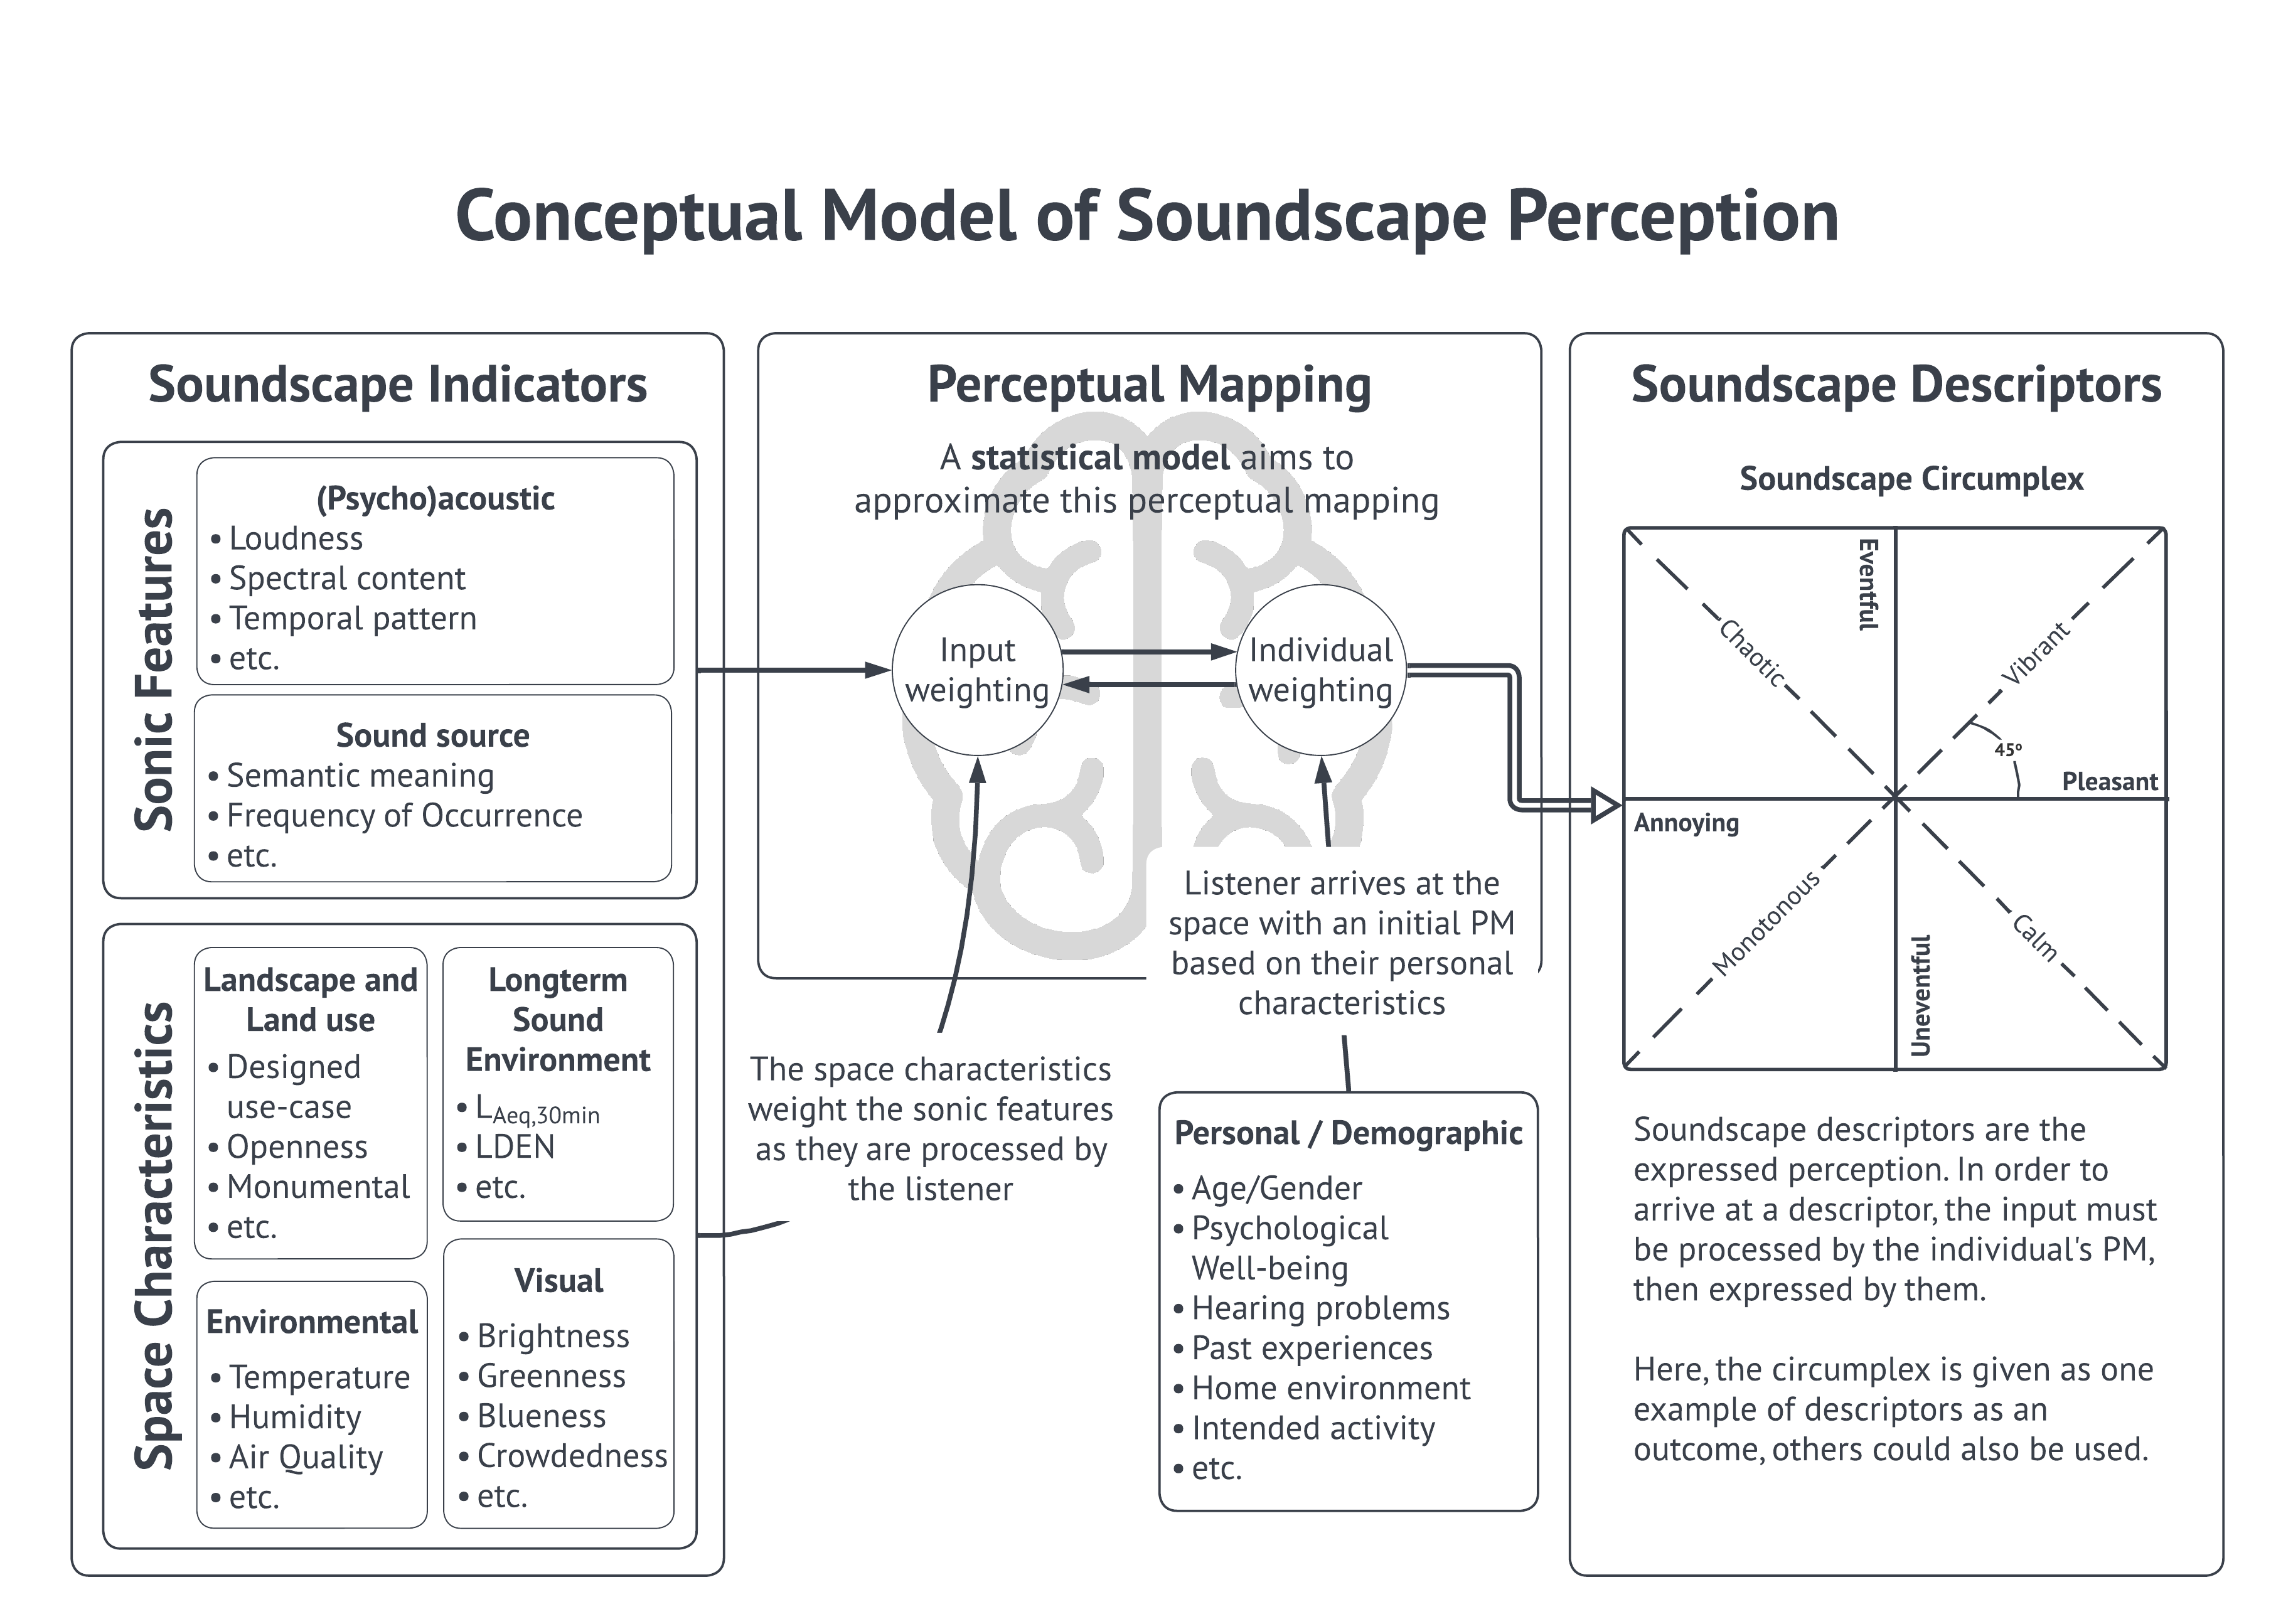
\includegraphics[width=\textwidth]{Figures/Overall Model Concept Diagram_2022-04-28.png}
  \caption{The conceptual model of soundscape perception, illustrating the perceptual mapping from physical inputs, through personal experience, to soundscape descriptors. The role of the statistical model is to attempt to approximate or reflect this perceptual mapping. \label{fig:percepMap}}
\end{figure}

\cref{fig:percepMap} shows a conceptual view of this relationship. We start with \textbf{soundscape indicators}, describing the physical environment to which a listener is exposed. Soundscape indicators characterise the physical and contextual environment to which the listener is exposed. This can be broken down into \textbf{sonic features} (e.g. the acoustical features listed above) and \textbf{characteristics of the space} itself (e.g. the amount of visible sky, the intended use-case of the space, how crowded the space is, etc.). In order to translate from the physical inputs to an expressed description of the soundscape perception, we introduce the concept of a \textbf{perceptual mapping} \citep{Lionello2021Thesis}. This mapping represents a simplified idea of how each individual's brain processes the inputs from the soundscape which they experience, forms a perception, and finally expresses that perception through their description of the soundscape. For our purposes, this perceptual mapping is treated as essentially a black box mapping inputs to outputs. It can be conceived of as a network of weights in which certain characteristics of the sound may have different weights and directions depending on the context, through which all of the inputs are processed, resulting in the soundscape rating. Conceptually, this perceptual mapping -- the pathways and weightings through which the inputs are processed before being expressed as a perceptual descriptor -- is established prior to an individual's exposure to the soundscape in question.

We then break the perceptual mapping into two parts: how the inputs are weighted relative to each other (which is relatively consistent across participants) and the particular variation in each person's perception based on their own experiences and background. In this conceptual model, the weighting of the sonic features (both the acoustic features and the sound source information) are mediated by the space characteristics as they are processed by the listener. The individual weightings represent the effects due to the listener's particular personal characteristics (their age, gender, psychological well-being, etc.) as well as the inherent unpredictable randomness in each individual's experience of the soundscape.  Following the definition of soundscape established in \cref{sec:terminology}, the `soundscape' would be the general term used to describe all of the inputs to the perceptual mapping while the outcome of the perceptual mapping is the soundscape perception, as expressed through soundscape descriptors.

It should be made clear that this represents a very simplified view of how a soundscape perception is formed, however it provides a useful conceptual framework for the purposes of understanding and modelling how someone's perception forms in response to their exposure to a space. One way to consider the function of a statistical model of soundscape perception is as replicating the perceptual mapping between soundscape indicators and descriptors \citep{Lionello2021Thesis}. As a person experiences an urban space, they are exposed to an array of physical inputs, these are then processed by the listener through their own personal experience and mapped to their perception of that space. This perception is then expressed through their description of this experience of the soundscape. It is this mapping of physical inputs to perceptual description which the statistical model aims to reflect. The most successful model would then accurately replicate the general perceptual mapping across the population.

% As will be expanded upon in \cref{sec:NeedForPredModels}, the core message of this thesis is the importance of developing models which can predict soundscape perception and be put to use in assessing urban soundscapes. \citet{Aletta2016Soundscape} crucially laid out a forward-looking framework for the terminology used in soundscape studies and how the development of predictive models can progress. The work presented in this thesis can be viewed as fulfilling the steps presented in that framework and further developing Aletta's ideas around the creation and uses of predictive modelling. In line with this, the following section will review \citet{Aletta2016Soundscape} in depth in order to clarify the background which led to the advancements presented in \crefrange{ch:lockdown}{ch:ProbabilisticPOC}.


% In order to consistently discuss soundscape and the factors which influence it, it is important to understand what terms have been used to describe soundscapes. Both the traditional focus on the epidemiological impacts of noise and the development of the soundscape concept have used many different terms in order to describe the perception of a sound environment. Following \citet{Aletta2016Soundscape}, I'll group these under soundscape descriptors. 


\subsection{Perceived affective quality}
\label{sec:paqReview}
Based on the work in \citet{Aletta2016Soundscape} and a recent review of predictive soundscape models \citep{Lionello2020systematic}, among the potential soundscape descriptors which can be used, I have selected the soundscape circumplex \citep{Axelsson2010principal}, specifically the version in Method A of \citet{ISO12913Part2}, as the most appropriate for predictive modelling. 

Method A is built on a series of descriptors referred to as the \glsfirst{paq}, proposed by \citet{Axelsson2010principal}. These \glsplural{paq} are based on the pleasantness-activity paradigm present in research on emotions and environmental psychology, in particular Russell's circumplex model of affect \citep{Russell1980circumplex}. As summarised by Axelsson: `Russell's model identifies two dimensions related to the perceived pleasantness of environments and how activating or arousing the environment is.' This circumplex model is formed of two dimensions, pleasantness (often referred to as valence) and activity (or arousal), which are orthogonal to each other. In their study, three primary dimensions of soundscape perception were extracted from participants' responses to complex sound samples measured on 116 attributes, using Principal Components Analysis. The first component was found to represent pleasantness (aligning with attributes such as comfortable, appealing, uncomfortable, disagreeable, and inviting) and explained 50\% of the variance in the dataset. The second component was found to represent eventfulness (eventful, lively, uneventful, full of life, and mobile) and explained 18\% of the variance. The third component was found to represent familiarity (commonplace, common, and familiar) and explained 6\% of the variance, however this third component is typically disregarded as part of the standard circumplex. As will be made clear throughout, the circumplex model has several aspects which make it useful for representing the soundscape perception of a space as a whole.

When applied to soundscape, Axelsson re-termed these main axes as `Pleasant' and `Eventful', and also identified a set of additional axes which are rotated 45° from the main axes. This rotated axis contains additional attributes which represent various mixtures of the pleasant and eventful attributes: `Exciting', `Chaotic', `Monotonous', and `Calm'. This circumplex model of soundscape can be seen in \cref{fig:circumplexOnly}. In Method A, these \glsplural{paq} are collected through a series of questions with 5-point Likert-type responses where participants are asked to what extent they agree or disagree that the present surrounding sound environment is pleasant, exciting, etc. for each of the 8 descriptors. Method A also includes questions on: the sound source composition of the space, broken down into `Traffic noise', `Other noise', `Sounds from human beings', and `Natural sounds'; overall soundscape quality; and appropriateness of the sound environment to the place. The circumplex model, along with the sound source and general soundscape questions represent a relatively comprehensive method for assessing the soundscape of a space.

\begin{figure}
  \centering
  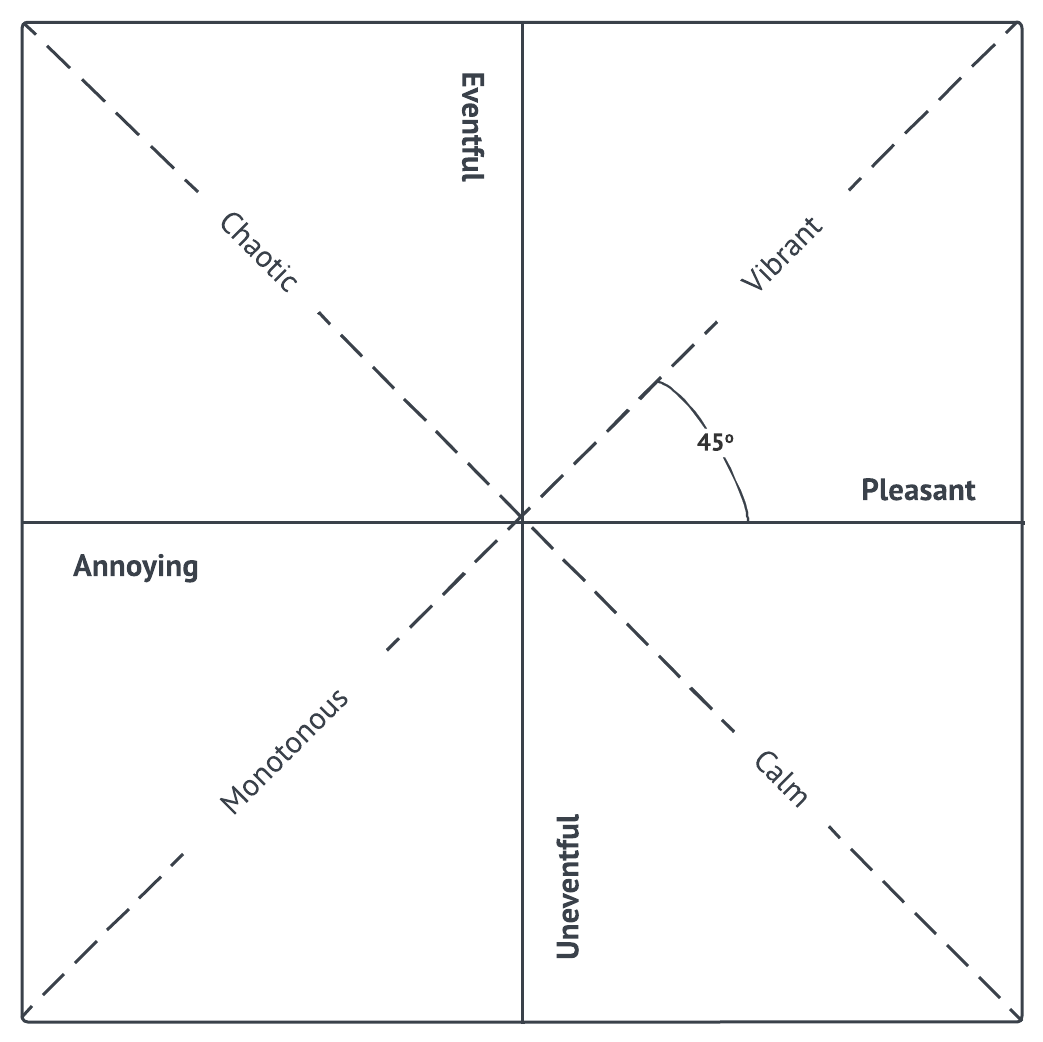
\includegraphics{Figures/CircumplexOnly.png}
  \caption{The soundscape circumplex, as originally derived by \citet{Axelsson2010principal} and updated in \citet{ISO12913Part2}. \label{fig:circumplexOnly}}
\end{figure}

One benefit of the circumplex model is that, as a whole, it encapsulates several of the other proposed soundscape descriptors - in particular, annoyance, pleasantness, tranquility, and possibly restorativeness \citep{Aletta2016Soundscape}. According to \citet{Axelsson2015How}, the two-dimensional circumplex model of perceived affective quality provides the most comprehensive information for soundscape assessment. It is also possible that the overall soundscape quality could itself be derived from the pleasant-eventful scores derived for a soundscape.

The circumplex also lends itself well to questionnaire-based methods of data collection, as proposed in \citet{ISO12913Part2}. In contrast to methods such as soundwalks, interviews, and lab experiments, in-situ questionnaires are able to provide the quality and amount of data which is necessary for statistical modelling. Large-scale, in-situ questionnaires are therefore considered the most appropriate data collection approach for generating a soundscape assessment database intended for predictive modelling. Combined, these factors make the circumplex most appropriate for predictive modelling as it provides a comprehensive summary of soundscape perception in a form which lends itself to machine learning model development.

\section{Statistical models of soundscape perception}
Several studies prior to the formalization of the ISO standards on soundscape demonstrated the general, but inadequate, relationship between traditional acoustic metrics, such as $L_{Aeq}$, with the subjective evaluation of the soundscape \citep{Berglund2006Tool,Yang2005Acoustic,Rychtarikova2013Soundscape,Aumond2017Modeling,AlsinaPages2021Perceptual}. These have typically aimed to address the existing gap between traditional environmental acoustics metrics and the experience of the sound environment. Yang and Kang (2005) showed that, when the sound level is `lower than a certain value, say 70 dBA', there is no longer a significant change in the evaluation of acoustic comfort as the sound level changes. However, the perceived sound level does continue to change along with the measured sound level, showing that (1) measured sound level is not enough to predict soundscape descriptors such as `acoustic comfort', and (2) there is a complex relationship between perceived sound level and soundscape descriptors which is mediated by other factors.

\citet{Ricciardi2015Sound} proposed two models based on data collected from a smartphone application to predict urban sound quality indicators based on linear regressions. The first model which incorporated perceptually-derived input features (visual quality and familiarity) achieved an $R^2$ of 0.72, while a second model without these features achieved an $R^2$ of 0.58. This indicates the necessity for considering and accounting for the influence which contextual factors in a space have on the relationship between the sound environment itself and the listener's perception of it (i.e. the soundscape) while also highlighting the challenges associated with a predictive model which depends only on measurable features.

% Subsequent studies have shown that, even with large data sets and several possible acoustic indicators examined, models that are based on objective/measurable metrics under-perform in predicting soundscape assessment when compared to models based on perceptual responses. \citet{Ricciardi2015Sound}, with a methodology based on smart phone recordings, achieved $R^2 = 0.21$ with acoustic input factors $L_{50}$ and $L_{10} - L_{90}$, whereas the same dataset and model building method achieved $R^2 = 0.52$ with perceptual input factors overall loudness (OL), visual amenity (VA), traffic (T), voice (V), and birds (B). This indicates that merely examining the acoustic level is not sufficient for predicting the assessed soundscape quality, and that additional objective factors and a more holistic and involved method of characterizing the environment is required. 

\subsection{Input weighting}

Contrary to the hopes expressed by \citet{Aletta2014Towards}, that `ideally there should be one acoustic indicator per dimension', the evidence from subsequent investigations and modelling attempts \citep{Lionello2020systematic} indicates this to be unlikely. There appears to be no reason we should think the perceptual dimensions should be reduced to a single acoustic indicator. The dimensions of soundscape represent complex perceptual concepts which we should expect to be composed of a multi-factor interaction between the input features. This necessary complexity  highlights the need for a more sophisticated machine learning approach in order to handle and interpret the interactions between the many input features which contribute to the formation of a soundscape perception.

According to a recent review of predictive soundscape models from \citet{Lionello2020systematic}, the degree of employing auditory and non-auditory factors in soundscape prediction varies, with some studies relying on contextual, personal/demographic \citep{Erfanian2021Psychological,Tarlao2020Investigating} or social media \citep{Aiello2016Chatty} data entirely to predict and generate soundscape features. Some methods also incorporate perceptually-derived features, such as subjective sound level and visual pleasantness as predictors \citep{Lionello2020systematic}. In general, these methods which incorporate perceptually-derived inputs achieve better accuracy rates than those which don't. However this information must also be obtained from people via a survey and therefore are unsuitable for predictive modelling where surveys are not possible. 

These previous studies have generally been limited by one or many of the following factors:

\begin{itemize}
  \item limited number or types of locations;
  \item limited responses sample size;
  \item no non-acoustic factors.
\end{itemize}
These factors generally limit the generalizability of their results beyond the investigated locations.

\paragraph*{Psychoacoustic Annoyance }Models for the prediction of annoyance based solely on a combination of psychoacoustic metrics have been previously proposed, with the most notable model based on psychoacoustic metrics proposed by \citet{PsychoacousticsfactsmodelsZwicker}. The authors provide definitions and the empirical basis behind a series of psychoacoustic metrics (loudness, roughness, sharpness, fluctuation strength), the specifics of which will be expanded upon in \cref{chap:methods}. Briefly, these metrics relate to specific psychophysical sensations which move beyond the strictly physical descriptions of sounds. Acoustical metrics such as \gls{lzeq} describe the physical characteristics of a sound, derived from the magnitude of the pressure changes induced by the sound. By contrast, psychoacoustical metrics attempt to relate these physical characteristics to the sensation they induce in humans. They therefore provide a more direct insight into how sounds are perceived and interpreted by a listener. 

Each of the proposed psychoacoustic metrics therefore attempts to describe one aspect of the sonic quality of the sound such that a sound can be broken down and described through some combination of these metrics. Zwicker and Fastl then propose a model which combines these metrics to quantitatively describe annoyance ratings obtained in psychoacoustic experiments. From \citet[p. 327]{PsychoacousticsfactsmodelsZwicker}:

\begin{quotation}
  Basically, psychoacoustic annoyance depends on the loudness, the tone colour, and the temporal structure of sounds. The following relation between psychoacoustic annoyance, \gls{pa} and the hearing sensations loudness, N, sharpness, S, fluctuation strength, F, and roughness, R can be given:

  \begin{equation}
    \label{eqn:pa1}
    PA \sim N( 1 + \sqrt{[g_1(S)]^2 + [g_2(F, R)]^2})
  \end{equation}

\end{quotation}

\noindent{where $g_1()$ and $g_2()$ are functions of sharpness and fluctuation strength \& roughness, respectively.}

Based on the results of psychoacoustic experiments, the authors expand on this theory to provide the following general model of psychoacoustic annoyance:

\begin{equation}
  PA = N_5 ( 1 + \sqrt{w^2_s + w^2_{FR}})
\end{equation}

with 

\begin{itemize}
  \item \gls{n5} percentile loudness in sone
  \item $w_s = (\frac{S}{acum} - 1.75) * 0.25 \log{(\frac{N_5}{sone} + 10)}$ for $S > 1.75$ acum
\end{itemize}

describing the effects of sharpness S and 

\begin{itemize}
  \item $w_{FR} = \frac{2.18}{(N_5/sone)^{0.4}} (0.4 * \frac{F}{vacil} + 0.6 * \frac{R}{asper})$
\end{itemize}

describing the influence of fluctuation strength F and roughness R.


% \subsubsection*{Sound source information}
% \draft{Prob need more on sources}
% \citet{Brown1987Urban} presents a comprehensive (for 1987) review of urban noise assessments. They note that

% \begin{quote}
%   For most cities, the basic pattern of noise an be considered initially to be one which results from a network of roadway line source. The lower end of the hierarchy (local street sources) would be more correctly described as moving point sources. [\ldots] Superimposed on this pattern are the point sources such as industrial plants, air conditioners, animals, etc., again with a hierarchy of intensities but most with a sphere of influence much smaller than he noise from the roadway network.  
% \end{quote}

% A primary challenge with Brown's hierarchies here is their focus on the source; yes, there is a hierarchy in the degree to which any individual source exerts its influence on the surrounding environment. However, when we shift our focus away from the source and towards the receiver, we may see a different hierarchy form. A central aspect of the human-centred focus on soundscape is its movement away from a source focus towards a receiver focus. The source-focus is, as noted by Brown, a weakness in `traditional' noise assessment methods. 

\subsection{Individual weighting}
Several studies have attempted to study the degree to which personal and demographic factors influence a person's soundscape perception. In some conceptions \citep{Kou2020effects,Erfanian2019Psychophysiological} these personal factors are classed as 'contextual' soundscape indicators - features which influence or, in a modelling context, be used as independent variables to predict the value of a soundscape descriptor. The personal factors help to create a personal soundscape interpretation model which is individual to each person.

In this way, a person's individual state-of-mind, ethnic identity, educational background, gender identity, etc. form a pseudo-deterministic framework %! what a load of crap
through which the physical inputs from their environment are filtered. Clearly, many of these personal factors could never be measured and even those which are measurable will have wide ranges of legitimate effects. However estimating the degree and type of effect they may have can both help us better predict individual soundscape assessments and understand how group identities influence sound perception.

\section{An Engineering Approach: The need for predictive soundscape models}
\label{sec:NeedForPredModels}

The existing methods for soundscape assessment and measurement, such as those given in the ISO 12913 series, have been focussed primarily on determining the \emph{status quo} of an environment. That is, they are able to determine how the space is \emph{currently} perceived, but offer little insight into hypothetical environments. As such, they are less relevant for design purposes, where a key goal is to determine how a space \emph{will be} perceived, not just how an existing space is perceived. The methods for assessment outlined in \citet{ISO12913Part2} and for analysis given in \citet{ISO12913Part3} are inherently limited to post hoc assessments of an existing space. Since they are focussed on surveying people on their experience of the environment, it stands that the space must already exist for people to be able to experience. How then would an urban planner, architect, or other designer estimate how a potential user would react to a space which is under design and not available to be assessed? Toward this, and following from the combination of perceptual and objective data collection encouraged in \citet{ISO12913Part2}, the natural push from the design perspective is towards `predictive modelling'. In this context, predictive modelling involves predicting how physical acoustic environments would likely be perceived or assessed by the users of the space. 

The soundscape approach faces several challenges in practical applications which are unaddressed by current assessment methods, but which may be solved through the development of a predictive modelling framework. The first of these challenges is predicting how a change in an existing sound environment will be reflected in the soundscape. While it is possible in this scenario to measure the existing soundscape via questionnaire surveys, if a change is then introduced to the acoustic environment, it is so far impossible to say what the resulting soundscape change would be. This question relates strongly to the idea of soundscape interventions; where a particular noise pollution challenge is addressed by introducing more pleasant sounds (e.g. a water feature), following the soundscape principle of treating sound as a resource \citep{Lavia2016Soundscape}. Predicting how much a particular intervention would improve the soundscape (or, indeed whether it would improve at all) is not yet possible with the retrospective methods available. This question is also addressed in \cref{ch:lockdown} of this thesis which uses a predictive model to look at how the changes in the acoustic environment due to the COVID-19 lockdowns resulted in changes in the soundscapes of the spaces.

Retrospective assessment methods also struggle to capture the dynamics of the soundscape in a space. Whether through the narrative interview method of \citet[Sec. 5.4]{ISO12913Part2}, through soundwalks, or through in-situ questionnaires \citep{Mitchell2020Soundscape}, only the soundscape during the particular period which the researchers are actively investigating is captured. This makes it very difficult to determine diurnal, seasonal, or yearly patterns of the soundscape. These patterns may be driven by corresponding diurnal, seasonal, or yearly patterns in the acoustic or visual environment, or by variations in how people process and respond to the sound at different times of day/season/year. Currently the only way to investigate any of these patterns is through repeated surveys. Predictive modelling, on the other hand, could allow a trained soundscape model to be paired with longterm monitoring methods to track how a soundscape may change in response to changes in the acoustic environment.

Several studies have attempted to address this gap by developing machine learning or statistical models of soundscape perception which are focussed on prediction, rather than inference. An array of modelling techniques are used, with linear regression being the most common \citep{Lionello2020systematic}, and also including \glsfirstplural{ann} \citep{Yu2009Modeling,PuyanaRomero2016Modelling} and \gls{svr} \citep{Giannakopoulos2019Athens,Fan2016Automatic,Fan2017Emo}. However, these studies have focussed primarily on using these models to investigate the constructs of soundscape perception, with few efforts to put the models themselves to use. \cref{ch:lockdown} attempts to address this by both developing a predictive model and applying it to a practical scenario where traditional assessment methods were impractical.

\subsection{Soundscape mapping}
Similarly, a move towards modelling methods based on objective and/or measurable factors would facilitate the application of mapping in soundscape. While noise maps have become common in urban noise research and legislation \citep{EEA2020Environmental,Gasco2020Social}, they can be difficult to translate into a soundscape approach. The \glsfirst{end} \citep{Directive200249ECEuropeanUniEuropean}, first implemented in 2002, is the main EU instrument to identify noise pollution impacts and track urban noise levels across the EU. Its goals were to determine the population's exposure to environmental noise, make information on environmental noise available to the public, and prevent and reduce environmental noise and its effects. In general, noise maps are based on modelled traffic flows, from which decibel levels are extrapolated and mapped, although interpolation and mobile measurement methods have also been recently developed \citep{Aumond2018Kriging}. Alternatively, they can be produced using longterm \glspl{slm} or sensor networks. While these methods have significant utility for tracking increases in urban noise levels and are important for determining the health and societal impacts of noise on a large scale, their restricted focus on noise levels alone limits their scope and reduces the potential for identifying more nuanced health and psychological effects of urban sound. 

Several studies have attempted to bring soundscape to urban noise mapping. The most notable of these attempts \citep{Aletta2015Soundscape,Hong2017Exploring,Aumond2018Probabilistic,Kang2018model} bring new, more sophisticated methods for mapping urban sound (not just noise levels). For instance, all four present methods which map the relative level of various sound sources, producing maps of the spatial distribution of bird sounds, human voices, water sounds, etc. In \citet{Aletta2015Soundscape,Hong2017Exploring} the mapping relied on soundscape surveys conducted in public spaces, then used interpolation methods and basic relationships to the measured noise levels to generate a map of the perceived soundscape over the entire study space. \citet{Kang2018model}, after starting with survey responses, attempted to create a prediction method which relied only on the audio recordings made in the space to create visual maps of the predicted soundscape perception (i.e. the \glsplural{paq} `pleasant', `calm', `eventful', `annoying', `chaotic', `monotonous'). According to the authors, the prediction and mapping model would follow three steps: (1) sound sources recognition and profiling, (2) prediction of the soundscape's perceptual attributes, and (3) implementation of soundscape maps. Unfortunately, from the paper, it appears that the prediction model results were not actually used for the mapping and, again, the survey responses from 21 respondents were interpolated to create the soundscape map. Their results indicated to how a predictive model could have been slotted into a mapping use-case, but this was limited by (1) the relatively poor predictive performance for several of the attributes, (2) the inability to automatically recognise sound sources, and (3) a very limited dataset in terms of sample size and variety of locations.

While the connection is not made to perception, \citet{Aumond2018Probabilistic} focussed on creating sound maps which can reflect the pattern of sound source emergences over time within a city. By stochastically activating varying sound sources across their map, they could map the percentage of time when a sound source emerges from the overall complex sound environment. If a predictive soundscape model which incorporates sound source information can be developed, then the same procedure which led to their sound source emergence maps could also feed the soundscape model, resulting in a map of predicted perception over time. 

The broader use-case and need for such soundscape models and maps was recently highlighted by \citet{Jiang2022Ten}, which opens the discussion for how the value and impact of soundscapes should be measured and what tools are needed to enable the valuation of policy interventions for soundscapes. In response to Question 5, the authors make the necessity of predictive soundscape models quite clear:

\begin{quote}
  \textbf{Question 5: What soundscape metrics and data will be needed?}

  Answer: Quantitative soundscape metrics that link subjective perceptions to objective acoustic and contextual factors will be needed, to enable monetisation while at the same time account for the perception-based nature of soundscape.\\
 \ldots\\
Despite the varied requirements for soundscape metrics and data between and even within valuation methods, a standardised metric or set of metrics, such as dB in noise valuation [\ldots] will allow comparison and integration of different studies and building compatible evidence bases. In this respect, standardised soundscape data collection, reporting and analysis methods have been developed and suggested (ISO, 2018; 2019), and the data outputs, such as the two soundscape dimensions based on affective quality ratings, have the potential to be used as standardised soundscape metrics for valuation purposes.

  \begin{flushright}
    \citet{Jiang2022Ten}
  \end{flushright}
\end{quote}

Urban scale noise mapping and its implementation at the international level has been crucial in highlighting the health impacts of urban noise and in providing evidence for the negative cost of excess noise. Traffic flow models of noise, large community noise surveys, and policy requirements to track noise levels have all been necessary to reveal these impacts. By creating predictive soundscape models, combined with new tools and sensing capabilities from smart city efforts, we can bring soundscape into these same realms. Without this, these large-scale impact studies will be limited to valuing the negative cost of urban noise, missing the potential value of positive soundscapes. By bringing perception-based practice to the same scale and type of evidence, we can expand urban sound research to consider a holistic view of urban spaces and their impacts.

% It was a combination of research highlighting the health impact of noise \citep{Ising2004Health}, economic impacts of urban noise \citep{Bristow2014International,Galilea2005Valuing} and international-level noise monitoring and mapping efforts which led to the eye-opening statistics showing the true impact of urban noise with which I opened this thesis \citep{EEA2020Environmental}. By creating improved methods and tools which enable the same scale and type of evidence, we can allow research to investigate the full impact of urban sound beyond just its negative, noise-focussed impact, and do so at city- and country-level scales.

% The ability to predict the likely soundscape assessment of a space is crucial to implementing the soundscape concept in practical design. Current methods of assessing soundscapes are generally limited to a post-hoc assessment of the existing environment, where users of the space in question are surveyed regarding their experience of the acoustic environment \citep{Engel2018Review, Zhang2018Effect}. While this approach has proved useful in identifying the impacts of an existing environment, designers require the ability to predict how a change or proposed design will impact the soundscape of the space. To this end, a model that is built upon measurable or estimate-able quantities of the environment would represent a leap forward in the ability to design soundscapes and to assess their broad impacts on health and wellbeing.

\subsection{Conclusion}
Soundscape perception, while primarily driven by sound level, is mediated heavily by non-acoustic factors which interact with the sound level, spectral information, and temporal acoustic behaviour in complex ways. The soundscape is influenced by several levels of factors: the immediate and long-term acoustic environment, other environmental factors (e.g. temperature, air quality), the physical / visual characteristics of the space, the type of architectural space, and even cultural and country-level expectations. When approached in a predictive model context, the acoustic data must form the core components, but a coherent framework for describing how the influence of the acoustic factors is affected by the non-acoustic factors is required.

Simpler analyses have taken a fragmented approach, for instance where separate acoustic-factor models are built independently for each type of architectural space considered in the data set and, separately, statistical models are built to investigate another non-acoustic factor, e.g. visual greenness vs lack of greenness. In order to properly extract the influences of all of these levels of factors as well as to build a generalisable model which can be used in practice, this fragmented approach should be combined into a single multi-level model.

My research makes use of in-person field questionnaires, long-term manned questionnaires, and multi-factor characterisation of the environment as part of the ERC-funded project Soundscape Indices (SSID) and in further collaboration with the DYNAMAP project to collect this database across a wide range of locations and soundscape types. These datasets and their creation will be discussed in detail in \cref{chap:protocol,ch:mlmann}.

% This approach is unique in that it:
% \begin{enumerate}
%   \item fundamentally incorporates all identified factors of soundscape perception in a coherent manner;
%   \item is extensible and interpretable;
%   \item considers how soundscape change over both multi-hour and multi-day timescales and incorporates this dynamic behaviour for increased accuracy.
% \end{enumerate}

%%%%%%%%%%%%%%%%%%%%%%%%%%%%%%%%%%%%%%%%

% \draft{======== What is meant by `an engineering approach?=========}

% \begin{quote}
%   The engineering sciences, therefore, can be understood as aimed at the creation and control of physical-technological phenomena through technological means. The epistemic task is scientific \emph{knowledge for how to} do this. This knowledge concerns the physical-technological phenomena, including the technological devices that can be understood in terms of desired functional and undesired dysfunctional phenomena.
%   \begin{flushright}
%     \citet[pg. 85]{Boon2021Routledge}
%   \end{flushright}
% \end{quote}

% \begin{quote}
%   In the engineering sciences, education in \emph{mathematical} modeling of phenomena and technological systems is strongly developed. Several mathematical approaches can be distinguished (e.g., Dym 1980/2004). The most rudimentary approach starts from reproducibly measured, quantitative datasets and aims to find mathematical patterns or structures in them, represented by an algorithm, such as linear or exponential equations (considered \emph{phenomenological} laws such as Boyle's law or Hooke's law) or a set of equations that forms a mathematical model for a specific phenomenon or system.
%     \begin{flushright}
%     \citet[pg. 87]{Boon2021Routledge}
%   \end{flushright}
% \end{quote}

% \citet{Franssen2021Routledge} makes a compelling argument for 1) why quantitative metrics are necessary for an engineering approach; and, simultaneously 2) that a design's physical performance is not what matters, but the \emph{assessment} of that performance, `so it is this assessment which needs to be quantitative'. 


% \draft{========================}

